\documentclass[xetex, onlymath, handout]{beamer}
\usefonttheme{serif}
\usetheme{hsr}

% use lmodern for math
\usepackage{lmodern}

% math packages
\usepackage{amsmath}
\usepackage{amssymb}

% use plex font for monospaced, roboto for the rest
\usepackage[T1]{fontenc}
\usepackage{plex-otf} % monospaced
\usepackage{roboto} % other
\renewcommand*\familydefault{\sfdefault}

\usepackage{graphicx}
\usepackage{booktabs}
\usepackage{array}

% links
\usepackage{hyperref}
\hypersetup{
  % Remove ugly boxes
  hidelinks,
  % Set colors
  colorlinks = true,
  anchorcolor = black,
  citecolor = black,
  filecolor = black,
  linkcolor = black,
  menucolor = black,
  runcolor = black,
  urlcolor = {black!50!blue}, 
}

% pretty drawings
\usepackage{forest}
\usepackage{circuitikz}
\usepackage{tikz}
\usetikzlibrary{%
  calc,
  positioning,
  backgrounds,
  decorations.pathreplacing,
  decorations.markings,
  matrix,
  arrows,
}

\usepackage{pgfplots}
\pgfplotsset{compat=1.15}

% source code
\usepackage{listings}
%% create a lstlisting style
\lstdefinestyle{samplestyle}{
  belowcaptionskip=\baselineskip,
  breaklines=true,
  frame=none,
  inputencoding=utf8,
  % margin
  xleftmargin=\parindent,
  % background
  backgroundcolor=\color{hsr-lightgrey20},
  % default language:
  language=[LaTeX]TeX,
  showstringspaces=false,
  % font
  basicstyle=\ttfamily\small,
  identifierstyle=\color{hsr-black},
  keywordstyle=\color{hsr-blue},
  commentstyle=\color{hsr-black40},
  stringstyle=\color{hsr-mauve80},
}

\lstdefinelanguage{BibTeX}
  {keywords={%
      @article,@book,@collectedbook,@conference,@electronic,@ieeetranbstctl,%
      @inbook,@incollectedbook,@incollection,@injournal,@inproceedings,%
      @manual,@mastersthesis,@misc,@patent,@periodical,@phdthesis,@preamble,%
      @proceedings,@standard,@string,@techreport,@unpublished%
      },
   comment=[l][\itshape]{@comment},
   sensitive=false,
}

%% and set the chosen style
\lstset{style=samplestyle, escapechar=`}

% logos
\usepackage{hologo}


% metadata
\title{\textbf{Advanced} \textrm{\LaTeXe} Workshop}
\author[NaoPross]{\texttt{Naoki Pross --- np@0hm.ch}}
\date{Spring Semester 2022}

\institute[OST]{OST FHO Campus Rapperswil}
% \logo{
\includegraphics[width=3cm]{figs/hsr-logo}}

\AtBeginSection[]
{
  \begin{frame}
    \frametitle{Table of Contents}
    \tableofcontents[currentsection]
  \end{frame}
}


\begin{document}

\frame{
  \maketitle
}

\begin{frame}{I lied to you \textsuperscript{sorry}}
  \begin{center}
    \begin{tikzpicture}
      \begin{axis}[
        smooth, samples = 100,
        axis lines = left,
        axis line style = { thick },
        width = \textwidth,
        height = \axisdefaultheight,
        grid style = dashed,
        xlabel = Complexity,
        ylabel = Difficulty,
        x label style={at={(axis description cs:1,.1)},anchor=east},
        ytick = \empty,
        xtick = {2, 4, 6, 11, 13, 16, 20, 22},
        xticklabels = {Text, Figures, Tables, Math, Plots, {Technical\\ Report}, Thesis, Book},
        xticklabel style = {align = center},
        x tick label style = { rotate = 70, anchor = east, font=\footnotesize },
        legend style = { legend pos = north west, legend cell align = left },
        no markers, domain = 0:25,
      ]
        \plot[very thick, hsr-mauve60, domain=0:14]{exp(x/3 - 2.5)};
        \addlegendentry{Word}
        \plot[very thick, hsr-blue, dashed]{3/(1 + exp(-2*(x-2.5))) + x/50*exp((x-4)/12)};
        \addlegendentry{\textrm{\LaTeX}}
        \plot[very thick, hsr-blue]{3/(1 + exp(-2*(x-2.5))) + x/50*exp((x-4)/12) + 2/(1 + exp(-2*(x-16)))};
        \addlegendentry{Good \textrm{\LaTeX}}
      \end{axis}
    \end{tikzpicture}
  \end{center}
\end{frame}

\begin{frame}{Goals for today}
  \Large
  \begin{itemize}
    \item Organize your \textrm{\LaTeXe} code because your last document was an \emph{absolute fucking mess}
    % \item Understand \emph{why the hell} the compiler is complaining
    \item Consume your precariously short existence trying to learn to draw pictures with a terrible programming language called \emph{TikZ}
  \end{itemize}
\end{frame}

% \begin{frame}{About this presentation}
%   \begin{block}{Content}
%     \begin{itemize}
%       \item \textrm{\LaTeX} is \emph{learn by doing} \\
%       \item Will be mostly examples
%       \item Sorry for the crowded slides
%     \end{itemize}
%   \end{block}
% 
%   \begin{exampleblock}{Example}
%     Things in green boxes are examples
%   \end{exampleblock}
% 
%   \begin{alertblock}{Tip}
%     Things in red boxes are tips or extras
%   \end{alertblock}
% \end{frame}

\begin{frame}{Do yourself a favor}
  \begin{alertblock}{Use the International US Keyboard Layout}
    \centering
    \vspace{3pt}
    % 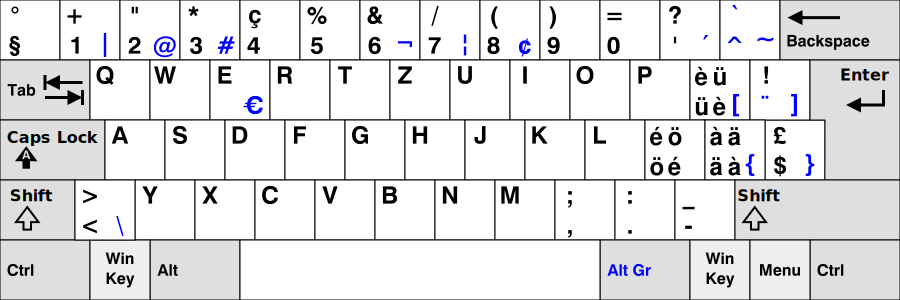
\includegraphics[height=9em]{figs/kbd-sg}
    % \\[5pt]
    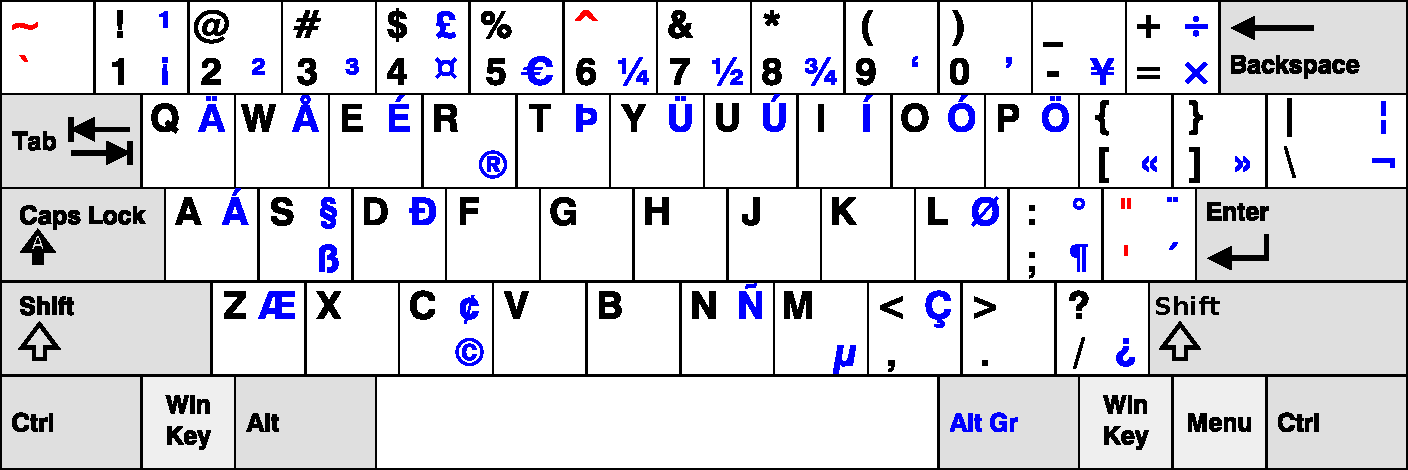
\includegraphics[height=9em]{figs/kbd-us-intl}
  \end{alertblock}
\end{frame}

\section{Absolute Basics to not ruin the typesetting}

\begin{frame}{Please enter the 21\textsuperscript{th} century}
  \begin{columns}
    \begin{column}{.2\textwidth}
      \begin{figure} \centering
        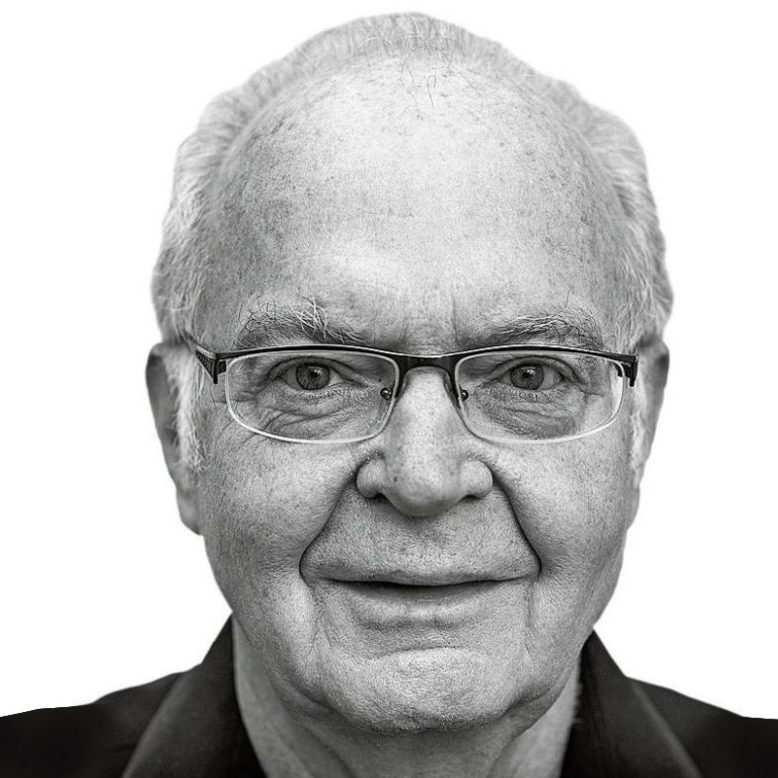
\includegraphics[height=8em]{figs/knuth}
      \end{figure}
      \begin{figure} \centering
        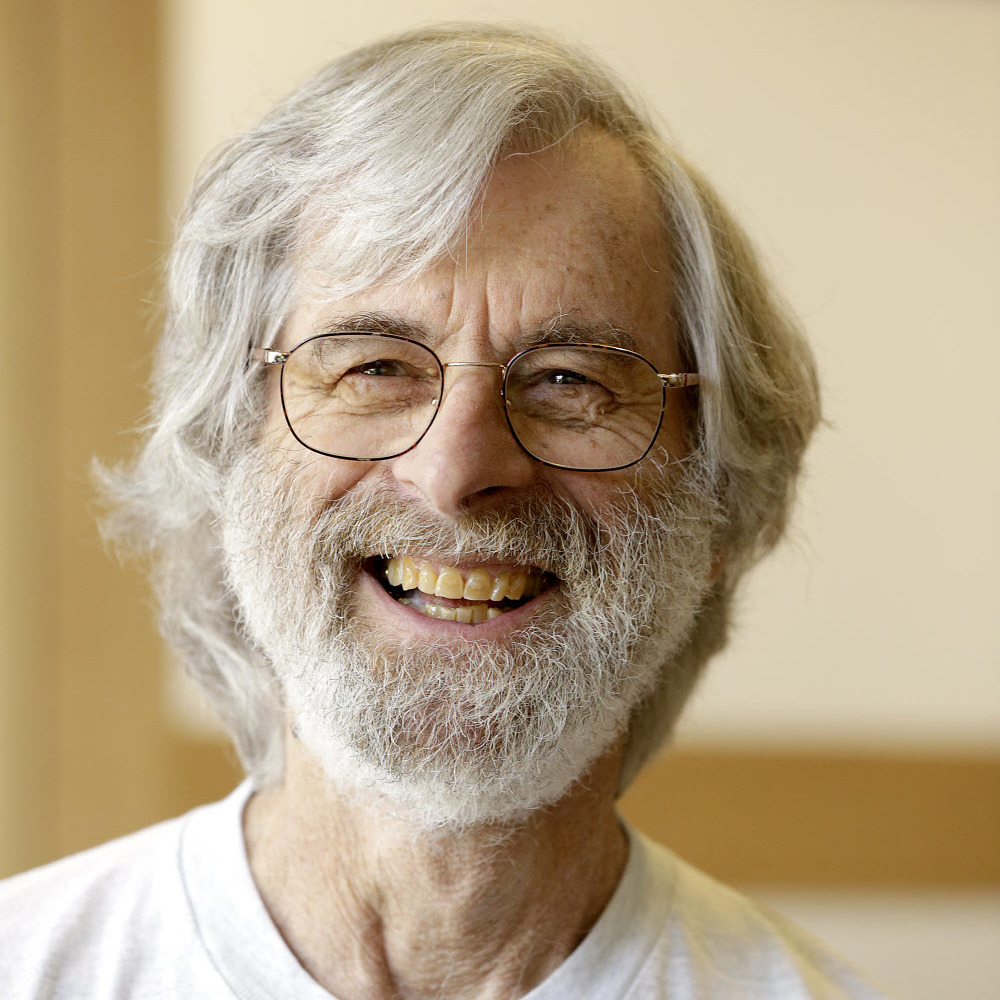
\includegraphics[height=8em]{figs/lamport}
      \end{figure}
    \end{column}
    \hfill
    \begin{column}{.8\textwidth}
      \begin{figure} \centering
        \begin{tikzpicture}
          \tikzset{
            block/.style = {
              draw, thick, rectangle,
              minimum height = 1cm,
              minimum width = 2cm,
              rounded corners,
              fill = hsr-lightgrey20,
            }
          }

          \node[block, fill=hsr-mauve20] (TEX) at (2.5,2) {\textrm{\TeX}};
          \node[right] at (TEX.east) {1978};

          \node[block, color=hsr-black40, fill=hsr-lightgrey20] (CONTEXT) at (-1,.5) {\textrm{\hologo{ConTeXt}}};
          \node[right, color=hsr-black40] at (CONTEXT.east) {1996};

          \node[block] (XETEX) at (0,-2) {\textrm{\hologo{XeTeX}}};
          \node[left] at (XETEX.west) {2004};
          \node[block] (LATEX) at (2.5,-1) {\textrm{\LaTeX}};
          \node[left] at (LATEX.west) {1984};
          \node[block] (LUATEX) at (5,-2) {\textrm{\hologo{LuaTeX}}};
          \node[left] at (LUATEX.west) {2007};

          \draw[thick, ->] (TEX) to[out=-90, in=90] (LATEX);
          \draw[thick, ->] (TEX) to[out=-90, in=90] (XETEX);
          \draw[thick, ->] (TEX) to[out=-90, in=90] (LUATEX);
          \draw[thick, ->, draw=hsr-black40] (TEX) to[out=-90, in=90] (CONTEXT);

          \node[block, fill=hsr-blue20] (XELATEX) at (1,-4) {\textrm{\hologo{XeLaTeX}}};
          \node[block, fill=hsr-blue20] (LUALATEX) at (4,-4) {\textrm{\hologo{LuaLaTeX}}};

          \draw[thick, ->] (XETEX) to[out=-90, in=90] (XELATEX);
          \draw[thick, ->] (LATEX) to[out=-90, in=90] (XELATEX);

          \draw[thick, ->] (LUATEX) to[out=-90, in=90] (LUALATEX);
          \draw[thick, ->] (LATEX) to[out=-90, in=90] (LUALATEX);

        \end{tikzpicture}
      \end{figure}
      \begin{center}
        A: Use \textrm{\hologo{XeLaTeX}}, it has UTF-8 support! (\"a, \"u, \^o, \ldots)
      \end{center}
    \end{column}
  \end{columns}
\end{frame}

\begin{frame}[fragile]{Line breaks}

  {\LARGE \bfseries Stop putting line breaks everywhere.}

  \begin{alertblock}{Don't}
    \begin{lstlisting}
%% wrong
This is a sentence in the first paragraph. \\
This is another paragraph.
    \end{lstlisting}
  \end{alertblock}

  \begin{block}{Do}
    \begin{lstlisting}
This is a sentence in the first paragraph.

This is another paragraph.
    \end{lstlisting}
  \end{block}

  Use \lstinline!\\! only in \lstinline!tabular!

\end{frame}

\begin{frame}[fragile]{Don't do manual styling}

  \begin{alertblock}{Don't}
    \begin{lstlisting}
I want that \textbf{this part} stands out.
    \end{lstlisting}
  \end{alertblock}

  There is an \emph{emphasis} macro

  \begin{block}{Do}
    \begin{lstlisting}
I want that \emph{this part} stands out.
    \end{lstlisting}
  \end{block}

  \href{https://github.com/HSR-Stud/Willkommen/blob/master/Guidelines.md#text-and-structure}{Click here} if you want to change how \lstinline!\emph! looks like.

\end{frame}

\begin{frame}[fragile]{Don't do manual styling, again!}

  {\LARGE \bfseries Never manually create headings}
  
  Yes, I've seen it done.

  \begin{alertblock}{Don't}
    \begin{lstlisting}
% NEVER do this
\textit{\textsf{My custom heading}} \\[1em]
    \end{lstlisting}
  \end{alertblock}

\end{frame}

\begin{frame}[fragile]{Customize headings}

  \begin{exampleblock}{With the \texttt{titlesec} package}
    \begin{lstlisting}
% in the preamble
\usepackage{titlesec}

\titleformat{\paragraph}[hang]
  {\normalfont\itshape\sffamily}
  {\theparagraph}{1em}{}

% later in the document
\paragraph{My custom heading}
    \end{lstlisting}
  \end{exampleblock}

  \begin{block}{}
    KOMA classes have their own customization commands
  \end{block}
\end{frame}

\begin{frame}[fragile]{Stop making ugly tables}

%   \begin{table}
%     \centering
%     \begin{tabular}{l >{\(}l<{\)} >{\(}l<{\)}}
%       \toprule
%       \bfseries Coordinates & \textbf{Volume } dv & \textbf{Surface } d\vec{s}\\
%       \midrule
%       Cartesian & - & dx\,dy     \\
%       Polar     & - & rd\,rd\phi \\
%       Curvilinear & - & |\mathbf{J}_f|\,du\,dv \\
%       \midrule
%       Cartesian   & dx\,dy\,dz                         & \uvec{z}\,dx\,dy     \\
%       Cylindrical & r\,dr\,d\phi\,dz                   & \uvec{z}r\,dr\,d\phi \\
%                   &                                    & \uvec{\phi}\,dr\,dz  \\
%                   &                                    & \uvec{r}r\,d\phi\,dz \\
%       Spherical   & r^2\sin\theta\, dr\,d\theta\,d\phi & 
%         \uvec{r}r^2\sin\theta\,d\theta\,d\phi \\
%       Curvilinear & |\mx{J}_f|\,du\,dv\,dw & - \\
%       \bottomrule
%     \end{tabular}
%     \caption{Differential elements for integration.}
%   \end{table}

\end{frame}

\section{Packages and classes}

\begin{frame}[fragile]{What is a package?}
  \begin{figure}[H]
    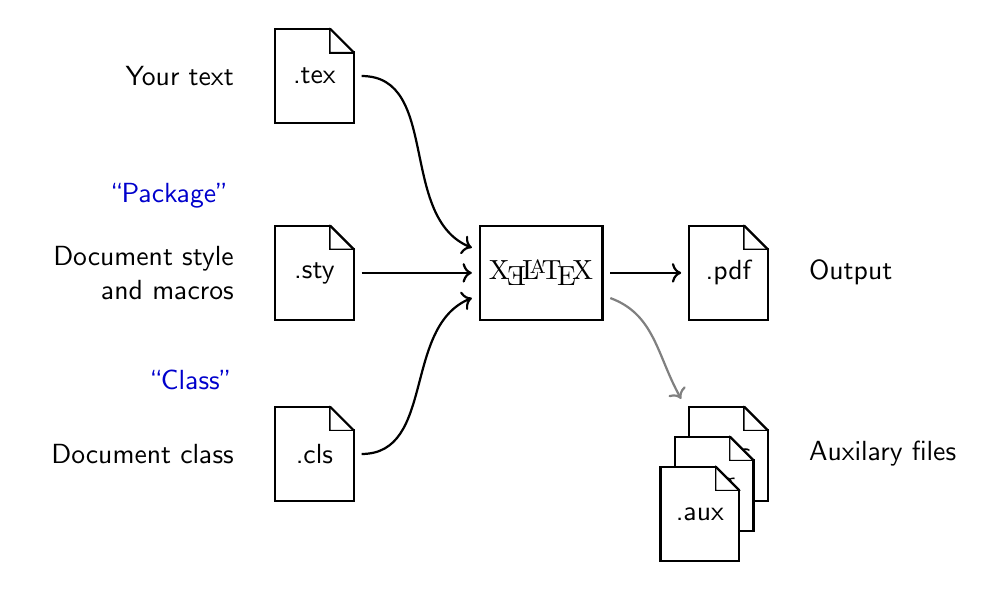
\begin{tikzpicture}[
        node distance = 1cm,
        pics/file/.style args = {#1 #2 #3}{
          code = {
            \node[
              outer sep = 0,
              inner sep = 0,
              minimum width = 1cm,
              minimum height = 1.2cm,
              #3
            ] (#1) {#2};
            \draw[
              thick, fill = white,
            ] ({#1}.north west) -- ($({#1}.north east) - (.3,0)$)
                -- ++(0,-.3) -- ++(.3,0) -- ({#1}.south east)
                -- ({#1}.south west) -- ({#1}.north west) -- cycle;
            \draw[
              fill = white,
            ] ($({#1}.north east) - (.3,0)$) to ++(0,-.3) to ++(.3,0) to ++(-.3,.3) to cycle;
            \draw[
              black, thick,
            ] ($({#1}.north east) - (.3,0)$) to ++(.3,-.3);
            \node[
              outer sep = 1mm,
              inner sep = 0,
              minimum width = 1cm,
              minimum height = 1.2cm,
            ] (#1) at (#1) {#2};
          }
        }
      ]

      \node[
        draw = black, thick,
        minimum height = 1.2cm,
        minimum width = 1.5cm,
        outer sep = 1mm,
      ] (C) at (0,0) {\textrm{\hologo{XeLaTeX}}};

      \draw pic{file = {STY .sty {left = 1.5cm of C}}}
            node[
              left = 3mm of STY,
              align = right,
              text width = 2.5cm
            ] {Document style and macros}
            node[
              above = 0mm of STY,
              anchor = south east,
              text width = 2.5cm,
              blue!80!black,
            ] {``Package''};
      \draw pic{file = {TEX .tex {above = 1.2cm of STY}}}
            node[
              left = 3mm of TEX,
              align = right,
              text width = 2.5cm
            ] {Your text};
      \draw pic{file = {CLS .cls {below = of STY}}}
            node[
              left = 3mm of CLS,
              align = right,
              text width = 2.5cm
            ] {Document class}
            node[
              above = 0mm of CLS,
              anchor = south east,
              text width = 2cm,
              blue!80!black,
            ] {``Class''};


      \draw[thick, ->] (TEX.east) to [out = 0, in = 160] (C);
      \draw[thick, ->] (STY.east) to [out = 0, in = 180] (C);
      \draw[thick, ->] (CLS.east) to [out = 0, in = 200] (C);

      \draw pic{file = {PDF .pdf {right = 1cm of C}}}
            node[
              right = 3mm of PDF,
              text width = 2cm
            ] {Output};

      \draw pic{file = {TOC .toc {below = 1cm of PDF}}}
            node[
              right = 3mm of TOC,
              text width = 2cm,
            ] {Auxilary files};
      \draw pic{file = {LOG .log {below left = -13mm of TOC}}};
      \draw pic{file = {AUX .aux {below left = -13mm of LOG}}};

      \draw[thick, ->] (C) to (PDF);
      \draw[thick, gray, ->] (C) to[out = -20, in = 120] (TOC.north west);
    \end{tikzpicture}
  \end{figure}
\end{frame}


\section{TikZ ist kein Zeichenprogramm}

\begin{frame}[fragile]{What is TikZ}

{\Large\bfseries TikZ = TikZ ist kein Zeichenprogramm}
\begin{lstlisting}
\usepackage{tikz}
\usetikzlibrary{calc, positioning, ...}
\end{lstlisting}
\begin{lstlisting}
\begin{figure}
  \centering
  \begin{tikzpicture}[
      % global settings / styles
    ]

    % drawing commands

  \end{tikzpicture}
  \caption{... \label{fig:...}}
\end{figure}
\end{lstlisting}
\end{frame}

\begin{frame}[fragile]{Elements}

  {\bfseries Basics}
  \begin{itemize}
    \item \lstinline!\coordinate (name)  at (x,y);!
    \item \lstinline!\node[options] (name)  at (x,y)  {label};!
    \item \lstinline!\draw[options] commands;!
    \item \lstinline!\fill[options] commands;!
  \end{itemize}

  {\bfseries Drawing commands}
  \begin{itemize}
    \item Line \lstinline!(A)  -- (B)!
    \item Horiz. then vert. line \lstinline!(A)  -| (B)!
    \item Vert. then horiz. line \lstinline!(A)  |- (B)!
    \item Quadratic B\'ezier \lstinline!(A) ..  controls (P)  and (Q)  .. (B)!
    \item Advanced curve \lstinline!(A)  to[options] (B)!
    \item Nodes \lstinline!node[options] (name) {label}!
    \item Shapes \lstinline!(A) rectangle (B)!, \lstinline!(A) circle (2cm)!
  \end{itemize}
\end{frame}

\begin{frame}[fragile]{Basic example}
  \begin{columns}
    \begin{column}{.75\linewidth}
      \begin{lstlisting}
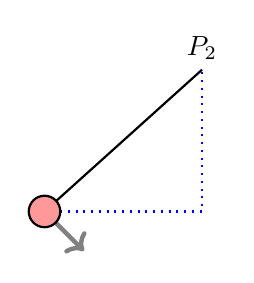
\begin{tikzpicture}
  \coordinate (O) at (0,0);
  \coordinate (A) at (2cm,18mm);
  % no units = cm

  \draw[thick] (O) -- (A);
  \draw[thick, dotted, blue] 
    (O) -| (A);

  \draw[ultra thick, ->, gray]
    (O) -- ++(5mm, -5mm);

  \fill[thick, draw = black,
    fill = red!40] (O) circle (2mm);

  \node[above] at (A) {\(P_2\)};
\end{tikzpicture}
      \end{lstlisting}
    \end{column}
    \begin{column}{.25\linewidth}
      \centering
      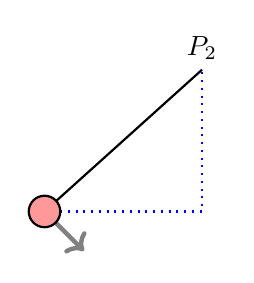
\begin{tikzpicture}
        \coordinate (O) at (0,0);
        \coordinate (A) at (2cm,18mm);
        % no units = cm

        \draw[thick] (O) -- (A);
        \draw[thick, dotted, blue] 
          (O) -| (A);

        \draw[ultra thick, gray, ->]
          (O) -- ++(5mm, -5mm);

        \fill[thick, draw=black,
          fill=red!40] (O) circle (2mm);

        \node[above] at (A) {\(P_2\)};
      \end{tikzpicture}
    \end{column}
  \end{columns}
\end{frame}

\begin{frame}[fragile]{Example with nodes}
  \begin{columns}
    \begin{column}{.8\linewidth}
      \begin{lstlisting}
\node (A) at (0,0) {A node};

\node[
  rectangle, very thick,
  draw = black, fill = green!20,
  font = \bfseries\slshape,
  % positioning library
  below = 5mm of A,
] (B) {Boxed};

\node[
  circle, thick,
  draw = black, fill = magenta!20,
  below = 1cm of B,
] (C) {\(m\)};

\draw[very thick, gray, ->]
  (C.east) to[bend right] (B.south east);
      \end{lstlisting}
    \end{column}
    \begin{column}{.2\linewidth}
      \centering
      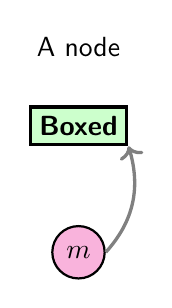
\begin{tikzpicture}
        \node (A) at (0,0) {A node};

        \node[
          rectangle, very thick,
          draw = black, fill = green!20,
          font = \bfseries\slshape,
          below = 5mm of A,
        ] (B) {Boxed};

        \node[
          circle, thick,
          draw = black, fill = magenta!30,
          below = 1cm of B,
        ] (C) {\(m\)};

        \draw[very thick, gray, ->]
          (C.east) to[bend right] (B.south east);
      \end{tikzpicture}
    \end{column}
  \end{columns}
\end{frame}

\begin{frame}[fragile]{TikZ V: Matrix and scope}
  \begin{columns}
    \begin{column}{.8\linewidth}
      \begin{lstlisting}
\matrix (M) [ % node with table of nodes
  row sep = 8mm,
  column sep = 4mm,
  nodes = {
    circle, thick,
    draw = black,
    fill = magenta!30,
    outer sep = 1mm,
  },
]{
  \node (A) {A}; & \node (B) {B}; \\
  \node (X) {X}; \\
};

\begin{scope}[ultra thick, gray, ->]
  \draw (X) -- (A);
  \draw (X) to[out = 0, in = -90] (B);
\end{scope}
      \end{lstlisting}
    \end{column}
    \begin{column}{.2\linewidth}
      \centering
      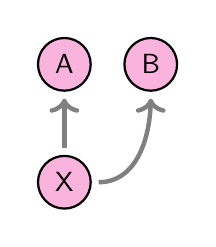
\begin{tikzpicture}
        \matrix (M) [
          row sep = 8mm,
          column sep = 4mm,
          nodes = {
            circle, thick,
            draw = black,
            fill = magenta!30,
            outer sep = 1mm,
          },
        ]{
          \node (A) {A}; & \node (B) {B}; \\
          \node (X) {X}; &               \\
        };

        \begin{scope}[ultra thick, gray, ->]
          \draw (X) -- (A);
          \draw (X) to[out = 0, in = -90] (B);
        \end{scope}
      \end{tikzpicture}
    \end{column}
  \end{columns}
\end{frame}

\frame{
  \centering
  \resizebox{!}{30pt}{
    {\Huge \bfseries\scshape The End}
  }
  \vspace{5mm}
  \newline
  {It wasn't worth the time I know, but hey, \newline
  at least now you know how to draw pretty pictures}
}

\end{document}

% vim:et:ts=2:sw=2:wrap:nolinebreak:
